

\documentclass[11pt]{article}
\setlength{\topmargin}{-.5in}
\setlength{\textheight}{9in}
\setlength{\oddsidemargin}{.125in}
\setlength{\textwidth}{6.25in}

 \usepackage{graphicx}
 \graphicspath{{images/}}
\begin{document}

\title{A User Model in Search for People with Autism}
\author{Esha Massand\\
MSc Computer Science Project Proposal\footnote{This proposal is substantially the result of my own work, expressed in my own words, except where explicitly indicated in the text. I give my permission for it to be submitted to the JISC Plagiarism Detection Service. }}
\date{\today}
\maketitle


\begin{abstract}
The current proposal presents my objective to research and build a user model within Search, to address the downfalls of current Search tools for individuals with Autism Spectrum Disorder (ASD). The user model will be built around the core features of ASD. The model will be applied to results returned from a synthesis of three leading existing search engines. The final product will be integrated with motion controllers, with the aim to enhance the user experience and the interface of Search for people with ASD.
\end{abstract}

\tableofcontents

\section{Introduction}
\subsection{Problem Statement}
Most search engines apply a general user model to refine search queries. The user models apply algorithms and weightings to each parameter, e.g., auto-complete, query understanding, site and page quality signals, user content and synonym snippets. No research to date has examined the experience of user search for individuals with Autism Spectrum Disorder (ASD), and whether these user models need to be adjusted for this subgroup. Although people with ASD are relatively proficient with technologies, we argue that the user models that underlie the way in which search queries are handled are different, and the needs of the user differ to the mainstream models. This project aims to build a suitable user model of ASD to address this gap.
As it has been shown that individuals with ASD are more engaged (show sustained attention) when using technology that is receptive (games, responsive consoles, motion controlled devices) and interactive compared to technology that is not, this project will combine interactive, Motion Recognition hardware with Search to improve the User Interface and architecture of Search for individuals with ASD.

\subsection{The Role of Context In Search}
It is unlikely that any given page on the web will contain a word or phrase that means exactly (or nearly) the same as another word or phrase in that language (e.g., shut and close). How is it then that your search engine of choice picks these phrases to mean the same thing, and returns them synonymously in the results of your query? Well, quite simply put, it is by virtue of the fact that each of their neighbouring words and associations are similar. These are indirect, higher-order associations, and provide the context in which the search engine can index keywords. This context plays a crucial role in search; first, in the interpretation of the query put forward by the user, and second, the context is reflected in the results returned to the user.

\subsection{What is ASD?}
The prevalence of Autism Spectrum Disorder (ASD) is amongst the most common neurodevelopmental condition and it is currently estimated that 1/68 children meet criteria for ASD (CDC, 2014). ASD is five times more common amongst boys than girls (1/42 boys, and 1/189 girls). According to the DSM-V (2013) diagnostic manual, ASD is characterized by persistent and early deficits in reciprocal social interaction and repetitive behaviours. Individuals vary from high functioning to low functioning (along a spectrum), with behaviours emerge around 2 or 3 years of age. 

\begin{center}
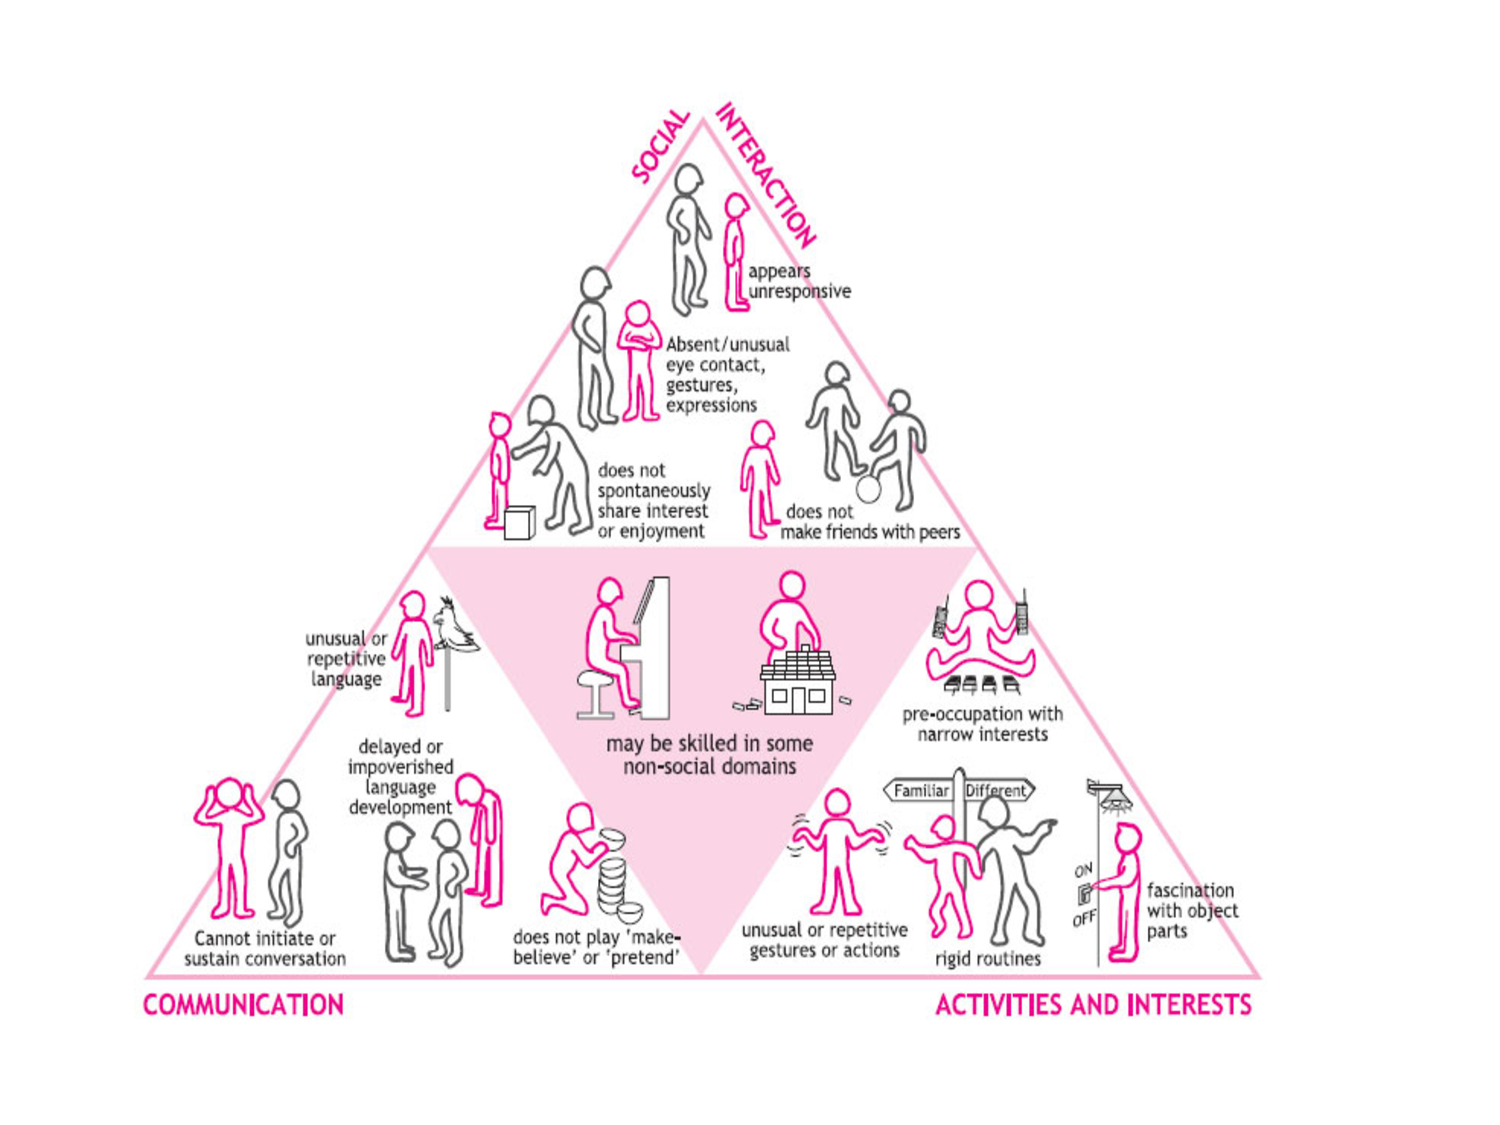
\includegraphics[scale=0.5]{asd}\\
The ASD Triad (source: http://media.kingdown.wilts.sch.uk/mod/page/view.php?id=7374)
\end{center}

\subsection{The Problem: Current Search Tools for people with ASD}
Search engines assume that the user is context-driven, and they attempt to model the user's intent using higher-order contextual information gathered from available web pages. This process also models the human brain's ability to extract context and semantic associations from information. However, what if the user was context-insensitive\footnote{Or, less context-sensitive}  and preferred a detail-focused processing style? They would intuitively form search queries very differently. For example, individuals with ASD are less likely to engage in a relational (hierarchically organized) style of processing (Bowler et al., 2009) suggesting that relating information in a hierarchically organised framework is less likely. Hierarchical organisation implies a great deal of flexibility and mental-shifting, as a simple example, in a search for 'apple', it would imply awareness that the word is related to 'pear' but also to 'fruit'. Awareness of this latter relation also suggests awareness that 'apple' is related to 'pomegranate'. Of course, in genuine search queries these associations can get very complex very quickly. Generally speaking, individuals with ASD prefer, and are more likely to engage in an item-specific processing style, and, whilst intelligent cognition is definitely possible, search queries are more likely formed of first-order associations\footnote{Of course there is a great deal of individual variability in Autism Spectrum Disorder.}. \\
\\Several Psychology learning and intervention studies for individuals with high functioning ASD have suggested that assimilation and accommodation of new information is most appropriate when:\\
\begin{enumerate}
\item Information is concrete (not abstract).\\
\item Information is presented in small manageable chunks.\\
\item Information is not verbally ?overloaded? (not too many words).\\
\item Information is presented in the expected way and does not deviate from this.\\
\\Several interventions have been built around this body of literature (www.autismspeaks.org).\\
Given these findings from the literature we can make several adjustments to current Search tools to enhance their benefit for people with ASD. For example, a user with ASD would have improved user-experience if their search results:\\
\item Were assessed (before presentation to the user) for the Key Word In a suitable Context.\\
\item Followed a similar order of semantic association, in line with the search query itself. \\
\item Were smaller and more manageable.\\
\item Were visually consistent.\\
\item Had a high degree of verbal consistency/similarity with the search query.\\
\end{enumerate}

\subsection{Proposal Organisation}

This proposal outlines my research to date on the field of Search, ASD, and User Interfaces. I also include my preliminary planning of the methods I will use to implement the enhanced Search tool for ASD. The remaining chapters discuss:
\begin{enumerate}
\item in Chapter X I give a brief introduction to Search engines, and the downfalls of current Search engines for individuals with ASD. I discuss the motivation behind the proposed work
\item in Chapter X I will discuss the existing combination/advanced search engines
\item in Chapter X I briefly discuss API?s and Libraries that I will use during the project, including Custom Search Engine APIs such as the Google Custom Search API, and Yahoo BOSS, Lucene Key Word In Context
\item in Chapter X I discuss the potential for user modeling within Search
\end{enumerate}



\section{What should Search offer people with ASD?}
\subsection{Search and Learning}
The Internet is one of the largest resources of information, and can be searched by users from different areas of the world relatively quickly. Search engines allow users to collate hundreds of links on a single topic, using only a few words or phrases. The variety of information returned is vast, and the depth of users’ searches can be determined by more advanced refinement options \footnote{For example, using the keyword NOT, or, by applying precedence to a selection of search query terms likely to be returned. This implies the user has some understanding of the keywords likely to be picked up and returned by the search engine. With this knowledge the user may choose to do a targeted search for just some specific key term.} . Search is an important learning tool; its significance is duly noted because of the learning benefits it brings for children and adolescents as they begin to navigate the Internet and gain an understanding of several subjects. 
Typically developing children are taught how to navigate search engines in school from a very young age (Google, Yahoo, Bing and other search engines), although other child-friendly searches exist (e.g., Ask Kids or KidRex). These child-friendly search engines’ aesthetics are designed specifically for children. They also prioritise the users ‘online safety’; in other words the results of the search have been filtered to include age-appropriate material, and they are visually presented in a more stimulating way for children.  Individuals with ASD represent a subset of the population who are not as engaged by interfaces of current search engines, like Google, Yahoo and bing, so they lose out on this important way to learn new information. The aim of the system is to be tailored to the needs of individuals with ASD, so that they do not lose out on this important learning tool.

\subsection{Clues from virtual reality and gaming}
Almost all teenagers (97\% of those aged 12-17) use a computer, web, portable or console devices, 73\% of which is desktop or laptop based. Teenagers with ASD also use technology and spend a substantial amount of their time using devices (Shane \& Albert, 2008). They are proficient, and use these devices with relative ease, showing high levels of engagement with consoles like the Xbox (Kinect) or Wii, Portable Gaming Devices (Nintendo DS), or cell phone or handheld device. For individuals with ASD, computer-based technologies can provide a stable, consistent learning environment that can be customized (Moore, McGrath \& Thorpe, 2000). The proposed system will utilize motion controllers (used by the Wii, Kinect) to facilitate engagement with Search. 

\subsection{Motion Controllers}
Motion recognition devices can be programmed to make consistent responses to environmental triggers. This is unlike real-world situations where environmental responses are not always consistent and may require further interpretation or ‘guess-work’. These controlled and interactive environments have shown promise for improving social communication skills and reducing repetitive behaviours (Games for Health, 2012).

\subsection{Visual not text-based}
People with ASD may prefer a more visually-oriented approach to search – one that doesn’t require sustaining a search query in working memory / attention and abstracting a question, to type it into a white box on a screen. It is likely that search can be just as powerful for learning and stimulating for them, if within an appropriate user interface that caters for these individuals needs.


\section {Creating a User Model of ASD}
\subsection{What is a user model?}
A user model is a collection of information associated with a particular user, with which a system can adapt its behavior in order to customize in line with the user’s needs. The concept of user modeling has strong implications for the way in which humans and computers interact; by creating a representation of the user, the system can be better informed about how to behave in various circumstances, for example, the system can acknowledge a specific kind of user’s needs, preferences, likes, dislikes, goals, plans, knowledge, and skill. The system can maintain this knowledge whilst interacting and adapting its behavior with the user.
Persona development will support the user modeling process by identifying particular characteristics of individuals with ASD in Search. An individual’s personal information pertaining to the persona, will be stored in a user profile which will contain information such as age, gender, lifestyle, frequent tasks, tools used, resources commonly used and crucially for this project, the profile will include information about diagnosis (Autism, Asperger, language ability).

\subsection{Types of user models}
User models can be static, and unchanging (i.e., no algorithms are used in order to teach the model about the changing preferences of the user, and no new information is fed into the model), or dynamic (representation of the user with their up-to-date changes in interests, and recent interactions with the system). Alternatively, user models can be stereotype
This means they utilize demographic information to classify users into distinct subtypes. The system infers or assumes other characteristics about this subset of users by making use of data gathered from other users also included within this subset. Lastly a user model can be highly adaptive and try to model the one user on their own, without stereotyping or inferring the characteristics of the user. This type of user modeling requires a large amount of data collection prior to its implementation.
\\The model can gather information through direct interaction with its user (e.g., via a registration process), by observing and interpreting the users actions, or, by a combination of both, that is, the system may ask for feedback, and alter its approach depending on the user’s behavior.

\subsection{Benefits and difficulties of user modeling in Search}
The model needs to collect data before it can predict the user’s needs with accuracy, but once this is achieved, information can be presented according to the user’s knowledge, ability and goals. It can also effectively filter out irrelevant information and rank the remaining search results in the most relevant way according for the user.
Creating a user model is not an easy task. The designer of the system has to set the weights of the parameters for the information that is fed into the model, and decide what course of action to take when two pieces of information may conflict. Some of the difficulties associated with deciding the priorities of elements of the model will be dealt with in a feasibility test (section X), and be refined with user-feedback /testing. Other elements of the user model will be based on modeling well-researched cognitive processes in ASD (for example, a user model that focuses on first-order, or, item-specific relations to form a search query, rather than hierarchical relations to form a search query).  

\subsection{Adaptive / Personalised Search}
Adaptive or Personalised search, is one way in which search engines including Google, Yahoo and Bing have attempted to tailor the search results for their users. The feature was first introduced as part of a GoogleLabs project in 2004 and implemented in 2005. It associates each user search with a HTTP cookie – this is a piece of data (a text file) sent from the website and saved in the users’ browser when the user navigates that website. These cookies contain information such as login information (gender, age), preferences (languages, interests) and other information about previous searches based on site traffic. The cookies allow the website to ‘remember’ stateful information about what buttons the user clicked on, or what sites they visited. This cookie record allows the search engine to return results that are highly relevant to the search query, but also highly relevant to the pages that the user visited through previous searches. When personalised or adaptive search is combined with GPS data from a smartphone or device, it can provide useful information about the places that user has previously visited to higher rank local items in the users returned results. This creates a personalized or adaptive web search, as the feature allows the web search to be tailored to the user’s preferences over the course of time, and as more searches are recorded.

\subsection{Disadvantages of adaptive search for individuals with ASD}
Although adaptive search seems to have significant user benefit in terms of relevance to the user for that search query, it decreases the likelihood that the user encounters new information and biases the results towards the users location and their previous site traffic.  This has the unwanted effect of creating a filter bubble (Pariser, 2011), which is argued to close us off from important and relevant information and create a personal ecosystem of information for one particular user, creating the impression that “our narrow self interest is all that exists”. The filter bubble also has potential privacy problems, as the user may be unaware that the search has been specifically tailored towards their interests and they wonder why things that they have previously searched for have become more and more relevant. The filter bubble may positively reinforce restricted interests in ASD as the user constantly receives feedback about their previous (idiosyncratic and personalized) searches without being able to break out of that repetitive loop. 
Recent research has suggested personalization also increases ‘background noise’ relative to the search results (Briggs, 2014). Briggs (2014) also suggests that there is a carry-over effect in personalized search for the users, whereby prior search results influence the results of subsequent searches \footnote{It should be noted that personalization of search results generally takes a lower priority for the ranking algorithms than the URLs ranked top in terms of their relevance for the search query.}.  Nevertheless this carry-over may be disadvantageous for people with ASD as it muddies their search space with previous interests, and provides unwanted distraction from the task at hand. 
It appears that in order to produce a search tool specifically tailored to reduce the filter bubble effect in ASD, widen the information gateway and reduce the possibility for restricted and repetitive searches, what is needed is a reprioritization of the weighting on previous search results in adaptive/personalized searches, in order to focus users on the current search at hand and limit the possibility that users get trapped in a spiraling loop of ever-narrowing user-relevant information and over personalization of self-reinforced information ecosystems.

\subsection{Where will the User Information be Stored?}

\section{Existing Combination/Advanced Search Engines}
No question about it, Google is still the world’s most popular search engine, and remains the most used search engine in the world (http://searchengineland.com/google-worlds-most-popular-search-engine-148089, 2013).  However, other highly capable search engines are being offered as alternatives, for example the Bing search engine offered by Microsoft, Yahoo, Ask, to name a few, and they deserve some exploration (http://www.makeuseof.com/tag/4-search-engines-that-combine-google-bing/).

\subsection{Bing vs Google}

\begin{center}
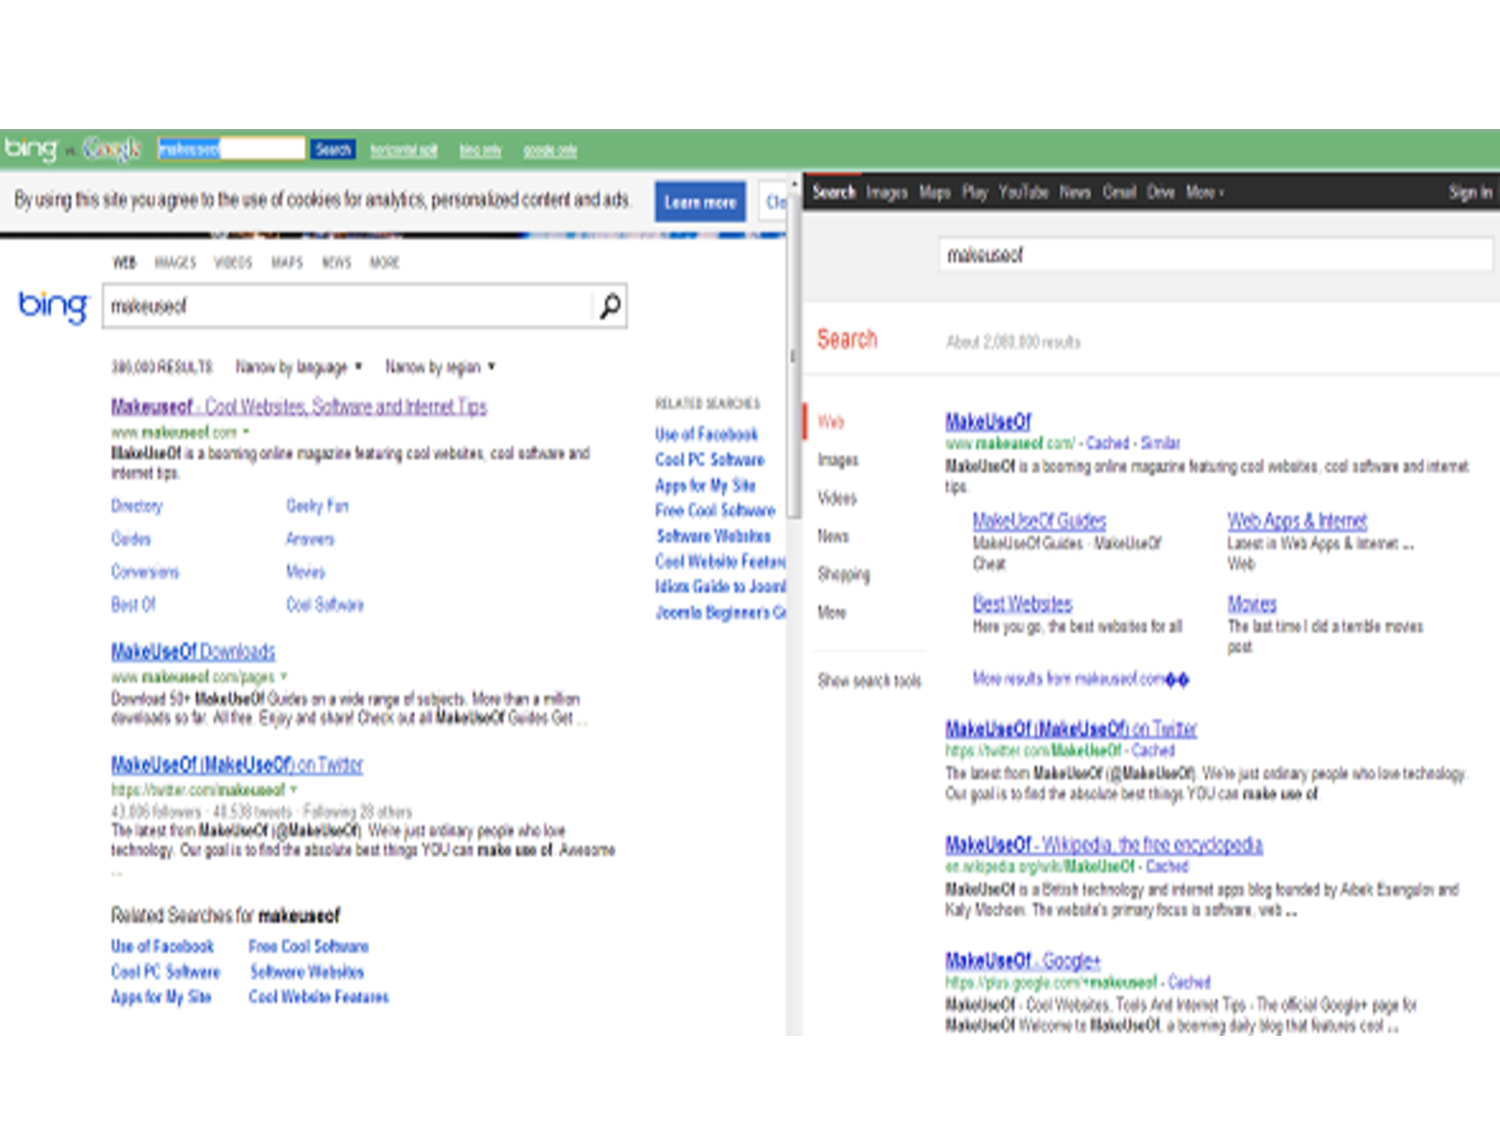
\includegraphics[scale =0.5]{bingG2}\\
Bing vs. Google presents the users’ search query results from both search engines to allow the user to make a comparison (the Google and Bing results can be presented vertically or horizontally beside each other), and provides the experience of navigating both search pages simultaneously.  The number of other personal preferences options is very limited (the orientation of the results is just about all the user has the option to choose).
\end{center}

\paragraph{Outline}
The remainder of this article is organized as follows.
Section~\ref{previous work} gives account of previous work.
Our new and exciting results are described in Section~\ref{results}.
Finally, Section~\ref{conclusions} gives the conclusions.

\section{Previous work}\label{previous work}
A much longer \LaTeXe{} example was written by Boney~\cite{Boney96}.

\section{Results}\label{results}
In this section we describe the results.

\section{Conclusions}\label{conclusions}
We worked hard, and achieved very little.

\begin{thebibliography}{100}

\bibitem {Boney96} Boney, L., Tewfik, A.H., and Hamdy, K.N., ``Digital
Watermarks for Audio Signals," \emph{Proceedings of the Third IEEE
International Conference on Multimedia}, pp. 473-480, June 1996.

\end{thebibliography}
\end{document}
